\documentclass[12pt, a4paper, openany]{book}
\usepackage[utf8]{inputenc}
\usepackage{graphicx}
\graphicspath{{assets/}}
\usepackage{float} % privides the H option

\title{\textbf{Data Structures and Algorithms Notes}}
\author{Venu Yeggadi}

\begin{document}
\maketitle

\tableofcontents

\chapter{Analysis of Algorithms}

\section{Commonly Used Fuctions}

 \subsection{The constant function}
The simplest function we can think of is the constant function, that is,
\[f (n) = c,\]
for some fixed constant c, such as c = 5, c = 27, or c = 210. That is, for any argument n, the constant
function f (n)  assigns the value c. In other words, it does not matter what the value of n is; f (n) will 
always be equal to the constant value c.

\subsection{The Logarithmic Function}
\[f(n) = \log_b n\] 
for some constant \(b > 1\).
\\* This function is defined as the inverse of a power, as follows:
\\*\(x = \log_b\) n if and only if \(b^x = n\).
\\*The value b is known as the base of the logarithm. Note that by the above definition,
for any base \(b > 0\), we have that \(\log_b 1 = 0\).
The most common base for the logarithm function in computer science is 2 as computers store integers
in binary. In fact, this base is so common that we will typically omit it from the notation when it is 2. That is, for us,
\[\log n = \log_2 n\]
\textbf{Logarithm Rules}: Given real numbers \(a > 0, b > 1, c > 0\),
and \(d > 1\), we have:
\\*1. \(\log_b(ac) = \log_b a+ \log_b c\)
\\*2. \(\log_b(a/c) = \log_b a -\log_b c\)
\\*3. \(\log_b(a^c) = c\log_b a\)
\\*4. \(\log_b a = \log_d a /\ log_d b\)
\\*5. \(b^{\log_d a} = a^{\log_d b}\)

\subsection{The Linear Function}
\[f (n) = n.\]
That is, given an input value \(n\), the linear function \(f\) assigns the value \(n\) itself.

\subsection{The \(n\log n\) Function}
\[f (n) = n\log n,\]
that is, the function that assigns to an input n the value of \(n\) times the logarithm base-two of \(n\).
This function grows a little more rapidly than the linear function and a lot less rapidly than the quadratic
function; therefore, we would greatly prefer an algorithm with a running time that is proportional to \(n\log n\),
than one with quadratic running time. An example is, the fastest possible algorithms
for sorting \(n\) arbitrary values require time proportional to \(n\log n\).

\subsection{The Quadratic Function}
\[f (n) = n^2.\]
That is, given an input value \(n\), the function \(f\) assigns the product of \(n\) with itself
(in other words, “\(n\) squared”).

\subsection{The Cubic Function and Other Polynomials}
\[f (n) = n^3,\]
which assigns to an input value \(n\) the product of \(n\) with itself three times.
The cubic function appears less frequently in the context of algorithm analysis
than the constant, linear, and quadratic functions
\\The linear, quadratic and cubic functions can each be viewed as being part of a
larger class of functions, the polynomials. A polynomial function has the form,
\[f (n) = a_0+a_1n+a_2n_2+a_3n_3 +\dots+a_dn_d,\]
where \(a_0, a_1, . . . , a_d\) are constants, called the coefficients of the polynomial, and
ad 6= 0. Integer d, which indicates the highest power in the polynomial, is called
the degree of the polynomial.

\subsection{The Exponential Function}
\[f (n) = b^n,\]
where \(b\) is a positive constant, called the base, and the argument n is the exponent.
That is, function \(f (n)\) assigns to the input argument \(n\) the value obtained by multiplying the base \(b\) by
itself \(n\) times. If we have a loop that starts by performing one operation
and then doubles the number of operations performed with each iteration, then the
number of operations performed in the \(n\)th iteration is \(2^n\).

\begin{figure}[H]
    \centering
    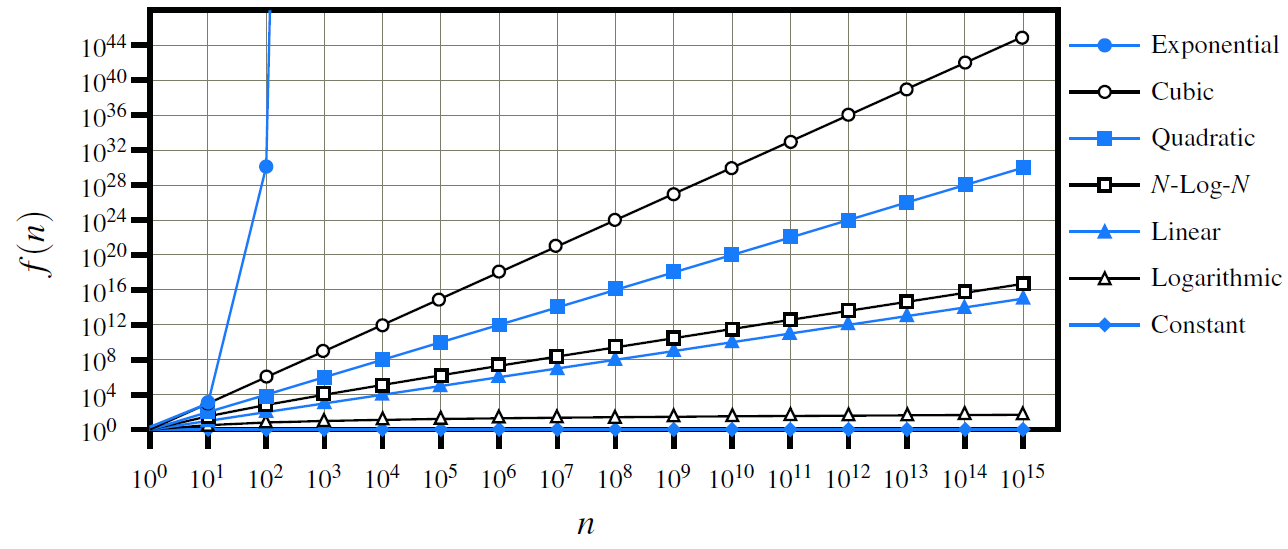
\includegraphics[width=1.2\textwidth]{AnalysisOfAlgorithms/ComparisonOfGrowthRates}
    \caption{Growth rates for the seven fundamental functions used in algorithm analysis.}
    \label{fig:ComparisonOfGrowthRates2}
\end{figure}


\section{The "Big O" Notation}
Let \(f (n)\) and \(g(n)\) be functions mapping positive integers to positive real numbers. We say that \(f (n)\) is 
\(O(g(n))\) if there is a real constant \(c > 0\) and an integer constant \(n_0 \geq 1\) such that
\[f (n) \leq c.g(n),\] for \(n \geq n_0\).
This definition is often referred to as the “big-Oh” notation, for it is sometimes pronounced
as “ f (n) is big-Oh of g(n).”

\begin{figure}[H]
    \centering
    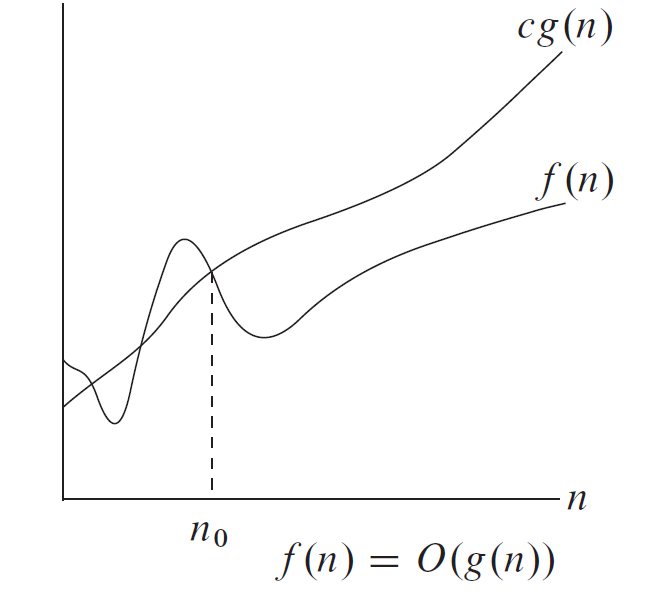
\includegraphics[width=0.5\textwidth]{AnalysisOfAlgorithms/BigOGraph}
    \caption{Illustrating the “big-Oh” notation. The function \(f (n)\) is \(O(g(n))\), since
\(f (n) \leq c.g(n)\) when \(n \geq n0.\)}
    \label{fig:BigOGraph}
\end{figure}

\textbf{Examples}
\\*Example: The function 8n+5 is O(n).
\\*Example: \(5n^4 +3n^3+2n^2 +4n+1\) is \(O(n4)\)
\\*Example: If \(f (n)\) is a polynomial of degree \(d\), that is, \(f(n) = a_0 +a_1n+···+a_dn^d\)
     and \(ad > 0\), then \(f (n)\) is \(O(n^d)\).
\\*Example: 
\\*Example: 
\\*Example: 
\\*Example: 
\end{document}